% PQSAFE-IL5-HYBRID-v1 — A crypto-agile post-quantum envelope for DoD file
% storage and transfer (a DoD SAFE-compatible replacement profile).
%
% Build:
%   latexmk -pdf pqsafe-il5.tex
\documentclass[11pt,a4paper]{article}
\usepackage{../shared/luxcover}
\usepackage[utf8]{inputenc}
\usepackage[T1]{fontenc}
\usepackage{amsmath,amssymb,amsfonts,amsthm}
\usepackage{graphicx}
\usepackage{hyperref}
\usepackage{booktabs}
\usepackage{algorithm}
\usepackage{algpseudocode}
\usepackage{listings}
\usepackage{xcolor}
\usepackage{tikz}
\usepackage{float}
\usepackage{enumitem}
\usepackage{array}
\usepackage{multirow}
\usepackage{tabularx}
\input{../shared/lstlang}
\usetikzlibrary{arrows.meta,positioning,shapes.geometric,fit,calc}

\hypersetup{colorlinks=true,linkcolor=black,citecolor=blue,urlcolor=blue}

\lstset{
  basicstyle=\ttfamily\scriptsize,
  breaklines=true,
  frame=single,
  numbers=left,
  numberstyle=\tiny\color{gray},
  keywordstyle=\color{blue!70!black}\bfseries,
  commentstyle=\color{green!50!black}\itshape,
  stringstyle=\color{red!60!black},
  showstringspaces=false,
}

\newtheorem{definition}{Definition}
\newtheorem{remark}{Remark}

\title{\textbf{PQSAFE-IL5-HYBRID-v1}\\
       \large A crypto-agile post-quantum envelope for DoD-grade\\
       file storage and transfer (a DoD SAFE compatibility profile)}
\author{Lux Industries Inc.\\
        \texttt{security@lux.network}\\
        \texttt{safe@apps.mil} (proposed)}
\date{Draft \today}

\begin{document}
\luxcoverpage
\maketitle

\begin{abstract}
PQSAFE-IL5-HYBRID-v1 is a crypto-agile envelope encryption profile for
DoD file storage and transfer designed to sit \emph{above} any approved
back-end (DoD SAFE, S3-compatible object storage, SharePoint, MinIO,
content-addressed stores, or the Lux storage chain) while ensuring those
back-ends never see plaintext, sender identity, recipient identity,
filenames, or classified metadata. The profile uses
\emph{hybrid}~\cite{xwing2024} post-quantum cryptography:
NIST-standardised
\textbf{ML-KEM-768} (FIPS~203~\cite{fips203}) combined with
classical X25519 via the IETF \textbf{X-Wing} construction~\cite{xwing2024};
\textbf{ML-DSA-65} (FIPS~204~\cite{fips204}) combined with classical
Ed25519 for sender authentication; and either AES-256-GCM (NIST CNSA
2.0~\cite{cnsa2}) or ChaCha20-Poly1305~\cite{rfc8439} for bulk AEAD chunk
encryption with sequence-numbered nonces and per-message forward
secrecy. Bulk data is never wrapped under the PQ key directly: the PQ
layer protects the \emph{file encryption key} (DEK), which protects the
file. Sender identity is bound through a hybrid PQ signature over a
canonical CBOR/COSE manifest~\cite{rfc8949,rfc8152}. \textbf{All X-Wing
and hybrid-identity primitives in PQSAFE come from the canonical Lux
package luxfi/zwing}~\cite{luxzwing} --- the same package provides the
Z-Wing secure channel for TCP/IP transport, so the bytes that encrypt
a file and the bytes that protect a session ride the same vetted
code path (one and only one X-Wing implementation; one and only one
hybrid-signature surface). Optional Reticulum Network Stack
(RNS, LP-9701~\cite{lp9701}) routing covers disconnected, mesh, or
LoRa deployments via the PQ-RNS profile in luxfi/pqrns~\cite{pqrns},
which itself rides zwing for identity + signing. The whole stack is FIPS/CNSA-2.0
aligned where validated modules exist and is explicitly \emph{crypto-agile
by design}: every algorithm, parameter set, KDF, AEAD, signature, and
manifest schema is versioned, so the profile can evolve to PQ-only when
DoD policy and PKI catch up. For everything the stack cannot send
end-to-end (replication, backup, legacy ingest), the same envelope is
re-keyed at rest using \textbf{luxfi/age} (age + ML-KEM-768
recipients~\cite{luxage}).
\end{abstract}

\tableofcontents

% ===========================================================================
\section{Threat model and design principles}
\label{sec:threat}

The defensible architecture for DoD is not ``replace DoD SAFE with
blockchain/PQ magic.'' It is:
\begin{quote}
\emph{Encrypt the file before it enters any storage or transfer system.
Sign the manifest. Audit every custody event. Keep keys off the
storage system. Make the PQ layer hybrid until policy, FIPS modules,
and PKI catch up.}
\end{quote}

PQSAFE-IL5-HYBRID-v1 inverts the usual ``trust the transport'' design:
DoD SAFE, object storage, Lux storage, or any other back-end is a dumb
ciphertext bucket. The crypto boundary is the sender's client, not the
storage system's TLS terminator.

\subsection{Adversaries}

\begin{itemize}[leftmargin=*,itemsep=0pt]
\item \textbf{Network adversary}: passive recorder + active
  store-and-decrypt-later attacker with future quantum computer.
  Defeated by ML-KEM-768 hybrid key wrap (X-Wing) on the envelope and
  ML-KEM-768 hybrid session establishment on the channel (Z-Wing).
\item \textbf{Storage adversary}: anyone with read access to the
  back-end (DoD SAFE database admin, S3 reader, ledger reader). Sees
  only ciphertext and minimal metadata. Cannot reconstruct plaintext
  without the recipient's long-term private key.
\item \textbf{Insider with key material}: a recipient may decrypt
  their own copy. The envelope binds recipient identity into the
  signed manifest so an unauthorised re-distribution is detectable;
  revocation is enforced through manifest expiry and a hash-only
  revocation registry.
\item \textbf{Endpoint compromise}: out of scope for the envelope.
  Mitigated by HSM-bound long-term keys, hardware roots of trust, and
  unattended-decryption being forbidden.
\item \textbf{Quantum adversary (CRQC)}: the entire stack is
  post-quantum on the confidentiality axis through ML-KEM-768. The
  authenticity axis is post-quantum through ML-DSA-65 with an
  SLH-DSA-192f long-term root option for high-assurance signing
  (LMS/XMSS available where stateful signing can be safely managed,
  per NIST SP~800-208~\cite{sp800208}).
\end{itemize}

\subsection{Non-goals}

\begin{itemize}[leftmargin=*,itemsep=0pt]
\item PQSAFE is \emph{not} a cross-domain solution. Classification
  boundaries are enforced outside the envelope.
\item PQSAFE does \emph{not} authorise recipients. It encrypts \emph{to}
  recipients chosen by an external ABAC/RBAC policy engine.
\item PQSAFE does \emph{not} store sensitive metadata on a public
  ledger. The Lux chain holds only opaque hash commitments.
\end{itemize}

\subsection{Principles}

\begin{enumerate}[leftmargin=*,itemsep=0pt]
\item \textbf{Hybrid first.} Every PQ primitive is paired with a
  classical primitive and combined with a KDF binding so the
  composition is at least as strong as the stronger of the two. This
  is the X-Wing construction~\cite{xwing2024} for KEMs and the
  ``classical + ML-DSA-65'' detached-signature pair for signatures.
\item \textbf{Symmetric for bulk.} Multi-GB files are encrypted with
  AES-256-GCM (FIPS-aligned, hardware-accelerated) or
  ChaCha20-Poly1305 (software-friendly fallback). The PQ primitive
  never wraps the bulk content; it wraps the DEK.
\item \textbf{Crypto-agile.} Every primitive carries a wire-byte
  identifier; manifests carry a profile-version field; the verifier
  routes by version. No alternate suites within a profile.
\item \textbf{Keys off the storage layer.} HSM-bound KEKs wrap
  per-file DEKs. Recipient public keys are certificate-bound.
  Recovery is M-of-N threshold, never a universal master decrypt key.
\item \textbf{Audit is tamper-evident, not secret-bearing.} Only
  hashes of envelope manifest, sender identity certificate, and the
  ordered recipient set go on the audit log.
\item \textbf{Forward secrecy at the channel layer; explicit policy
  for stored envelopes.} Z-Wing/PQ-RNS use ephemeral X-Wing per
  session and AEAD nonce sequence numbers so past sessions cannot be
  decrypted if a long-term identity key is later compromised.
  Stored envelopes target long-term recipient keys and therefore
  require complementary key-rotation, rewrap, revocation, and
  recovery policies (see Section~\ref{sec:pfs}).
\item \textbf{Domain separation everywhere.} Every HKDF and every
  signature carries an explicit context string identifying the
  protocol layer and version (e.g.\ \texttt{PQSAFE-MANIFEST-SIG-v1},
  \texttt{PQSAFE-DEK-WRAP-v1}, \texttt{PQSAFE-CHUNK-AEAD-v1}). No two
  layers ever derive a key from the same transcript.
\end{enumerate}

% ===========================================================================
\section{Cryptographic suite}
\label{sec:suite}

\begin{table}[H]
\centering
\small
\begin{tabularx}{\linewidth}{l l X}
\toprule
\textbf{Layer} & \textbf{Primitive} & \textbf{Standard / source} \\
\midrule
Bulk AEAD (FIPS profile) & AES-256-GCM & FIPS~197 + SP~800-38D~\cite{fips197} \\
Bulk AEAD (software profile) & ChaCha20-Poly1305 & RFC~8439~\cite{rfc8439} \\
Hash & SHA-384 / SHA-3-384 & FIPS~180-4 / FIPS~202 \\
Merkle hash & SHA-384 over 64-KiB chunks & this profile \\
KDF & HKDF-SHA-384 & RFC~5869 \\
Key wrap (hybrid KEM) & \textbf{X-Wing} = X25519 + ML-KEM-768 & IETF draft-connolly-cfrg-xwing-kem~\cite{xwing2024} \\
Key wrap (high-value) & X-Wing-1024 = X448 + ML-KEM-1024 & this profile \\
Sender signature (hybrid) & Ed25519 + ML-DSA-65 (detached pair) & RFC~8032 + FIPS~204~\cite{fips204} \\
Long-term root signature & SLH-DSA-SHA2-192f & FIPS~205~\cite{fips205} \\
Stateful root signature (option) & LMS-SHA-256-H10 & SP~800-208~\cite{sp800208} \\
Manifest format & CBOR/COSE & RFC~8949 + RFC~8152~\cite{rfc8949,rfc8152} \\
Channel (E2E PQ) & \textbf{Z-Wing} (X-Wing + Ed25519+ML-DSA-65 + ChaCha20-Poly1305) & luxfi/zwing~\cite{luxzwing} \\
File-at-rest envelope & luxfi/age + ML-KEM-768 recipient & age-encryption~\cite{age,luxage} \\
Mesh / LoRa transport (optional) & RNS hybrid PQ link & LP-9701~\cite{lp9701} \\
\bottomrule
\end{tabularx}
\caption{PQSAFE-IL5-HYBRID-v1 primitive stack.}
\end{table}

\subsection{Why X-Wing and not naive concatenation}

X-Wing~\cite{xwing2024} is a hybrid KEM that combines X25519 with
ML-KEM-768 through a SHA3-based KDF that binds the X25519 ephemeral
public key, the ML-KEM ciphertext, and a 6-byte label
\texttt{``\textbackslash{}.//\^{}'\textbackslash{}''} into the derived
secret. The construction is IND-CCA2 secure under \emph{either}
X25519's DH assumption or ML-KEM's M-LWE assumption: a break of one
component does not break the hybrid. Naive concatenation
$s = s_\text{X25519}\,\|\,s_\text{ML-KEM}$ is \emph{not} a KEM in the
strict KEM-API sense and is vulnerable to subtle re-encapsulation and
key-reuse pitfalls~\cite{xwing2024}. X-Wing fixes the API by emitting
a single ciphertext that captures both component ciphertexts and a
single 32-byte shared secret that's already KDF'd.

The IETF X25519MLKEM768 hybrid (IANA codepoint \texttt{0x11ec}) used
in TLS~1.3 is the same primitive at the cipher-suite level; the X-Wing
draft is the standalone construction for non-TLS protocols.

\subsection{Why ML-KEM-768 (not 1024) as the default}

ML-KEM-768 corresponds to NIST PQ Category~3 (security comparable to
AES-192) and is the production default for both Z-Wing and the file
envelope. ML-KEM-1024 (Category~5, AES-256-equivalent) is used for
high-value paths (recovery keys, KEK-wrapping-KEK, federation root).
Category~1 (ML-KEM-512) is not used: the marginal performance gain
does not justify diverging from the production default for an
operationally simple stack.

\subsection{Forward secrecy --- transport vs.\ stored envelopes}
\label{sec:pfs}

Transport forward secrecy and stored-envelope forward secrecy are
\emph{different problems with different solutions}. The paper makes the
distinction explicit so the security claim does not over-reach.

\paragraph{Transport (Z-Wing, PQ-RNS) --- full hybrid FS.}
For every session, both peers generate fresh X25519 and ML-KEM-768
ephemeral keypairs. After each session establishes its key, the
ephemeral private keys and any intermediate HKDF material are zeroed.
The session key derives from
$$K_\text{sess} = \textsf{HKDF-Extract-Then-Expand}\bigl(
\,\textsf{X25519}_\text{eph-eph}\,\|\,\textsf{ML-KEM-768}_\text{eph-eph}\,,\
\textsf{context}=\textsf{``ZWING-SESSION-v1''}\,\|\,H(\text{transcript})\bigr).$$
A future compromise of either long-term key (Ed25519 \emph{or}
ML-DSA-65) lets the adversary impersonate the identity going forward
\emph{but cannot decrypt previously recorded sessions}: the ephemeral
half is gone. Retrospective decryption requires recovering \emph{both}
classical and lattice ephemerals for every recorded link, which is
the hybrid FS contract. Long-term keys are used \emph{only} to
authenticate the ephemeral key-exchange transcript; they never directly
wrap session traffic.

\paragraph{Chunk AEAD --- intra-file FS via HKDF re-key.}
Each 64-KiB chunk is encrypted with a unique nonce
$(N_0\,\|\,\text{seq})$ where $N_0$ is a 12-byte random nonce-seed
bound into the manifest and $\text{seq}$ is a 4-byte big-endian chunk
index. The DEK itself is rotated every $2^{32}$ chunks (256~TiB) via
HKDF re-keying chained from the manifest's ratchet seed; compromise of
a re-keyed-DEK does not decrypt chunks emitted before the most recent
re-key. For interactive transfer this is irrelevant (files fit under
the rotation limit); for long-lived replication streams it prevents
one DEK compromise from leaking the entire history.

\paragraph{Stored envelopes --- DEK is wrapped to long-term recipient
keys, so naive FS does not apply.}
Each recipient's capsule wraps the per-file DEK under the recipient's
long-term X-Wing public key. If the recipient's long-term X-Wing
\emph{private} key is later compromised, every capsule that targeted
that recipient becomes decryptable, \emph{including capsules created
before the compromise}. This is the well-known property of any
recipient-targeted file-encryption scheme (PGP, age, S/MIME); it is
\emph{not} a defect of PQSAFE, but a property the operator must
manage. Five complementary controls reduce the residual risk:

\begin{enumerate}[leftmargin=*,itemsep=0pt]
\item \textbf{KMS/HSM-mediated unwrap.} Recipient long-term private
  keys live inside an HSM (Hanzo KMS / luxfi/kms). The HSM enforces
  policy at unwrap time (recipient identity, manifest TTL,
  revocation status, optional dual-control authorisation). A leaked
  recipient \emph{credential} (smartcard PIN) without HSM access
  does not unwrap capsules. The HSM is itself audit-logged.
\item \textbf{Short-lived recipient wrapping keys.} Recipients
  maintain a hierarchy: a long-term identity key (HSM-bound) and a
  shorter-lived wrapping subkey (rotated daily/weekly). Capsules
  target the wrapping subkey. Subkey expiry truncates the
  retrospective-decryption window if the subkey leaks.
\item \textbf{Epoch keys.} The wrapping subkey is parameterised by a
  monotonic epoch identifier $e$ ($1\text{ day}, 1\text{ week},
  1\text{ month}$, by policy). Capsules embed the epoch. Verifiers
  refuse capsules outside the active epoch window; the policy
  registry rotates the active set. An attacker who recovers an
  epoch-$e$ key can only decrypt envelopes sealed during epoch $e$.
\item \textbf{Rewrap-on-access (key rotation without re-encrypt).}
  When the recipient's wrapping key rotates, the sender (or a
  delegated rewrap service) re-encapsulates the DEK for each
  outstanding capsule under the new recipient key. The bulk chunks
  are untouched. Old capsules are deleted from storage; the
  ciphertext is now only decryptable by the new wrapping key.
\item \textbf{Threshold release.} Sensitive historical envelopes
  wrap the DEK under a Shamir-shared $(t, n)$ set of recipient
  keys. No single compromised recipient unwraps the DEK; $t$
  recipients must cooperate (see §\ref{sec:recovery}).
\end{enumerate}

\paragraph{Summary security statement.}
\emph{Confidentiality is provided by hybrid X-Wing key
establishment (X25519 + ML-KEM-768) with HKDF domain separation per
protocol layer. Authenticity is provided by detached hybrid
signatures (Ed25519 + ML-DSA-65) over canonical CBOR/COSE manifests
and transcript-bound capability negotiation. Bulk payload encryption
uses AES-256-GCM for the FIPS-oriented profile or ChaCha20-Poly1305
for the software profile, with sequence-numbered nonces, per-object
domain separation, and HKDF re-keying before nonce exhaustion.
Transport forward secrecy is provided when both classical and PQ
session secrets are ephemeral and erased after derivation; compromise
of long-term signing or identity keys does not decrypt prior sessions
but may enable impersonation until revocation. Stored envelopes use
DEK wrapping and require separate key-rotation, rewrap, revocation,
and recovery policy (see Section~\ref{sec:keys}).}

\subsection{Lamport / SLH-DSA / XMSS for the long-term root}

The profile signs every manifest with the sender's hybrid
Ed25519+ML-DSA-65 identity. The \emph{anchors} of that identity --
certificate authorities, policy registry roots, firmware signatures,
and the safe.apps.mil federation root -- are signed by SLH-DSA-192f
(stateless hash-based, FIPS~205) by default. SLH-DSA does not require
state tracking, which is operationally desirable for the federation
root. Where state tracking can be reliably enforced (e.g., an
air-gapped HSM with a counter), LMS-SHA-256-H10 or XMSS-SHA-256-H10
(SP~800-208) are alternates: smaller signatures, but stateful, so
each signing operation must be journaled or signatures will fly off
into compromise. For high-volume manifest signing we keep ML-DSA-65
(lattice, stateless, faster); for root-of-trust signing where the
signing rate is small, the stateless hash-based scheme is the
better fit.

% ===========================================================================
\section{Envelope format}
\label{sec:envelope}

A PQSAFE envelope is a directory or a single \texttt{.pqsafe} container
file containing:

\begin{verbatim}
report.pdf.pqsafe/
  manifest.cbor       - CBOR/COSE signed manifest
  manifest.sig        - Ed25519+ML-DSA-65 detached signature
  capsules/           - one per recipient
    01.cbor           - X-Wing(recipient_pub_xwing) -> wrap(DEK)
    02.cbor
    ...
  chunks/             - bulk ciphertext
    000001.bin        - AEAD(DEK, nonce_seed||1, chunk_1)
    000002.bin
    ...
  proof/              - optional Z-Chain inclusion proof
    inclusion.bin
\end{verbatim}

\subsection{Manifest schema (CBOR/COSE)}

\begin{lstlisting}[language=json,caption={Manifest schema (CBOR-decoded to JSON for readability).}]
{
  "profile":            "PQSAFE-IL5-HYBRID-v1",
  "manifest_version":   1,
  "created":            "2026-05-12T22:00:00Z",
  "ttl":                "168h",
  "policy_label":       "CUI",
  "policy_uri":         "policy://safe.apps.mil/policies/CUI-IL5-HYBRID-PQ-v1",
  "bulk_aead":          "AES-256-GCM",
  "hash":               "SHA-384",
  "kdf":                "HKDF-SHA-384",
  "kem":                "X-Wing-MLKEM768",
  "sig_classical":      "Ed25519",
  "sig_pq":             "ML-DSA-65",
  "chunk_size":         65536,
  "chunks": [
    {"index": 1, "len": 65536, "sha384": "..."},
    {"index": 2, "len": 65536, "sha384": "..."},
    ...
    {"index": 8421, "len": 14336, "sha384": "..."}
  ],
  "merkle_root":        "sha384:...",
  "nonce_seed":         "base64url:...",
  "envelope_id":        "sha384:...",          % bound AEAD AAD (see below)
  "sender": {
    "x509_chain_hash":  "sha384:...",
    "did":              "did:lux:...",
    "pq_pub_mldsa65":   "base64url:...",
    "pub_ed25519":      "base64url:..."
  },
  "recipients": [
    {
      "recipient_id":     "alice.mil",
      "pub_xwing":        "base64url:...",
      "capsule":          "capsules/01.cbor",
      "x509_chain_hash":  "sha384:..."
    },
    {
      "recipient_id":     "bob.gov",
      "pub_xwing":        "base64url:...",
      "capsule":          "capsules/02.cbor",
      "x509_chain_hash":  "sha384:..."
    }
  ],
  "audit": {
    "anchor_chain":     "lux-q",
    "audit_uri":        "https://audit.safe.apps.mil/v1/commits",
    "commit_hash":      "sha384:..."
  }
}
\end{lstlisting}

\subsection{Capsule format}

Each capsule wraps the per-file DEK for one recipient under that
recipient's X-Wing public key.

\begin{verbatim}
capsule.cbor = {
  "v":      1,
  "kem":    "X-Wing-MLKEM768",
  "kem_ct": <encoded X-Wing ciphertext (~1184 bytes)>,
  "aad":    sha384(manifest.cbor),
  "wrap":   AES-256-GCM(DEK, K_recipient, AAD=aad)
}
\end{verbatim}

The recipient executes:
\begin{enumerate}[leftmargin=*,itemsep=0pt]
\item Verify manifest signature (Ed25519 \emph{and} ML-DSA-65; both must
  pass).
\item Look up own capsule by recipient ID.
\item $K_\text{recipient}\,\gets\,\textsf{X-Wing.Decap}(sk_\text{xwing},\,
  \text{kem\_ct})$ -- this fails if either lattice or DH leg is corrupt,
  guaranteeing hybrid security.
\item $\textsf{DEK}\,\gets\,\textsf{AES-256-GCM-Open}(\text{wrap},\,
  K_\text{recipient},\,\text{aad})$.
\item Decrypt each chunk: $c_i\,\gets\,\textsf{AEAD.Open}(\textsf{DEK},
  \,\text{nonce\_seed}\,\|\,i,\,\text{ct}_i)$.
\item Verify Merkle root over chunk hashes matches manifest.
\end{enumerate}

\subsection{Envelope identifier and AEAD AAD binding}
\label{sec:envelope-id}

The chunk AEAD takes \texttt{envelope\_id} as additional authenticated
data so that ciphertext chunks cannot be lifted from one envelope and
replayed inside another. To make this binding itself verifiable the
identifier is computed up-front from inputs that are fully determined
before chunk encryption and is then carried inside the signed manifest:
\[
\textsf{envelope\_id}\;=\;\textsf{SHA-384}\bigl(\,
\texttt{profile}\,\|\,
\texttt{version}_{32}\,\|\,
\texttt{pub\_ed25519}\,\|\,
\texttt{pq\_pub\_mldsa65}\,\|\,
\texttt{nonce\_seed}\,\|\,
\texttt{created}\,\|\,
\bigl\|_{i}\,(\texttt{recipient\_id}_i\,\|\,\texttt{pub\_xwing}_i)
\bigr).
\]
At Open time the verifier recomputes \texttt{envelope\_id} from the
signed manifest fields and refuses if the recomputed value does not
byte-match the \texttt{envelope\_id} carried inside the manifest. The
manifest signature already covers \texttt{envelope\_id}, so any
attempt to substitute a different AAD is caught either by the
recomputation check or by the hybrid signature check.

\subsection{Algorithm allow-list at verify}
\label{sec:allow-list}

The manifest fields \texttt{hash}, \texttt{kdf}, \texttt{kem},
\texttt{sig\_classical}, \texttt{sig\_pq}, and \texttt{chunk\_size}
are not advisory. PQSAFE-IL5-HYBRID-v1 verifiers MUST refuse any
envelope whose manifest carries values other than the canonical set:
\texttt{SHA-384}, \texttt{HKDF-SHA-384}, \texttt{X-Wing-MLKEM768},
\texttt{Ed25519}, \texttt{ML-DSA-65}, and a \texttt{chunk\_size} of
\(65536\) bytes. New parameter sets land as a new profile string
(\texttt{PQSAFE-IL5-HYBRID-v2}, \dots), not as parameters inside v1.
This eliminates downgrade as a class.

% ===========================================================================
\section{Key management}
\label{sec:keys}

\begin{table}[H]
\centering
\small
\begin{tabularx}{\linewidth}{l l X}
\toprule
\textbf{Key} & \textbf{Role} & \textbf{Custody} \\
\midrule
DEK & per-file symmetric key (256 bits) & ephemeral, never persisted on storage system \\
KEK & wraps DEK at rest in storage layer (optional) & HSM/KMS (Hanzo KMS / luxfi/kms) \\
Recipient X-Wing & per-recipient hybrid PQ KEM keypair & user smart card / TPM / HSM; classical X25519 + ML-KEM-768 \\
Recipient signing & per-recipient hybrid sig keypair (Ed25519 + ML-DSA-65) & smart card / TPM; manifest counter-signatures, optional \\
Sender identity & per-sender hybrid sig keypair (Ed25519 + ML-DSA-65) & smart card / TPM; ALWAYS signs manifest \\
Federation root & SLH-DSA-192f keypair (FIPS~205) & air-gapped HSM; signs CA certs + policy registry \\
Recovery quorum & M-of-N threshold of recovery shares & distributed across agencies; rebuild DEK without single decryptor \\
\bottomrule
\end{tabularx}
\caption{Key roles and custody.}
\end{table}

\subsection{Recovery without a master key}
\label{sec:recovery}

PQSAFE forbids a universal master decrypt key. Recovery requires
threshold cooperation:

\begin{enumerate}[leftmargin=*,itemsep=0pt]
\item DEK is Shamir-shared $(t, n)$ at creation (typical: $t=3, n=5$ across
  agency CISOs) over $\textsf{GF}(2^{256})$.
\item Shares are wrapped under each share-holder's recipient X-Wing
  public key into capsules in the envelope's \texttt{recovery/}
  subdirectory.
\item Reconstruction requires $t$ share-holders to participate; no one
  party can decrypt unilaterally.
\item Audit log records every reconstruction event with the manifest
  hash, share-holder hashes, and timestamp.
\end{enumerate}

This matches LP-019 (Threshold MPC)~\cite{lp019} and uses the same
threshold signing kernel that the Lux primary network deploys for
QuasarCert: luxfi/corona (Ring-LWE) and luxfi/pulsar (Module-LWE)
threshold ML-DSA. The \emph{file} recovery quorum and the \emph{chain}
finality quorum share no key material, but they share the same Pedersen
DKG + proactive resharing lifecycle.

% ===========================================================================
\section{Transport: Z-Wing and RNS}
\label{sec:transport}

PQSAFE envelopes can be transferred over any channel; the envelope is
self-protecting. Two transport profiles are recommended:

\subsection{Z-Wing (TCP / IP)}

Z-Wing (\texttt{luxfi/zwing}~\cite{luxzwing}) is the canonical Lux
post-quantum secure channel. It exposes a \texttt{net.Conn} so
application protocols (file transfer, ZAP RPC, gRPC, HTTP/2, anything
that wants a stream) run unchanged on top.

\begin{table}[H]
\centering
\small
\begin{tabularx}{\linewidth}{l X}
\toprule
\textbf{Layer} & \textbf{Z-Wing v1} \\
\midrule
KEM & X-Wing (X25519 + ML-KEM-768) per the IETF draft~\cite{xwing2024} \\
Identity & Ed25519 + ML-DSA-65 hybrid signatures (FIPS~204) \\
AEAD & ChaCha20-Poly1305 with sequence-numbered nonces \\
Replay protection & 64-bit sequence counter; per-direction key derivation \\
Forward secrecy & Ephemeral X-Wing per session; long-term keys do not encrypt \\
Negotiation & None. Z-Wing v1 is one suite. \\
Layering & Routes over plain TCP today; RNS in v2 \\
\bottomrule
\end{tabularx}
\caption{Z-Wing channel surface.}
\end{table}

The ``no negotiation'' choice is deliberate. Cipher negotiation has
been the source of every major TLS downgrade attack. Two endpoints
either speak Z-Wing v1 or they don't talk. A future Z-Wing v2 (e.g.,
ML-KEM-1024 + Ed448 + ML-DSA-87) is a new ALPN-style identifier, not a
parameter inside v1.

\subsection{Reticulum Network Stack (RNS)}
\label{sec:rns}

For deployments where TCP/IP isn't available -- mesh radio, LoRa,
disconnected networks, contested EW environments -- PQSAFE rides over
RNS (LP-9701~\cite{lp9701}). RNS is a cryptographic-mesh transport
that uses identity-based addressing and hop-by-hop authenticated
encryption, originally designed for amateur radio and now widely
adopted by survival-mesh communities.

The Lux RNS profile (see \texttt{node/network/dialer/rns\_*.go}) keeps
RNS's classical identity (Ed25519 + X25519) and adds a hybrid PQ
identity layer parallel to Z-Wing's:

\begin{table}[H]
\centering
\small
\begin{tabularx}{\linewidth}{l X X}
\toprule
\textbf{Purpose} & \textbf{Classical (RNS native)} & \textbf{Post-quantum (Lux profile)} \\
\midrule
Identity signing & Ed25519 & ML-DSA-65 (FIPS~204) \\
Key exchange & X25519 & ML-KEM-768 (FIPS~203) \\
Session encryption & AES-256-GCM & -- \\
Key derivation & HKDF-SHA256 & -- \\
\bottomrule
\end{tabularx}
\caption{RNS hybrid PQ suite (LP-9701).}
\end{table}

Forward secrecy properties:
\begin{itemize}[leftmargin=*,itemsep=0pt]
\item Fresh X25519 + ML-KEM-768 keypairs per session.
\item Ephemeral private keys zeroed after the handshake completes.
\item Combined secret = $\textsf{HKDF}(\text{X25519 shared}\,\|\,
  \text{ML-KEM shared})$ -- both components must break to
  retrospectively decrypt.
\item AES-256-GCM session keys are rotated on RNS's standard ratchet
  cadence; nonces are sequence-numbered.
\end{itemize}

Wire-format growth from classical RNS to the PQ-hybrid profile:

\begin{table}[H]
\centering
\small
\begin{tabular}{l r r r}
\toprule
\textbf{Component} & \textbf{Classical} & \textbf{Hybrid} & \textbf{$\Delta$} \\
\midrule
Public identity & 64 B & $\sim$3.2 KiB & +3.1 KiB \\
Signature & 64 B & $\sim$2.5 KiB & +2.4 KiB \\
Key exchange ct & 64 B & $\sim$1.2 KiB & +1.1 KiB \\
Handshake total & $\sim$256 B & $\sim$7.5 KiB & +7.2 KiB \\
\bottomrule
\end{tabular}
\caption{Wire-format growth (per LP-9701 LP-9701 measurements).}
\end{table}

A capability-exchange byte in the announce frame advertises PQ
support. A peer with \texttt{requirePostQuantum: true} refuses
classical-only peers; a peer with \texttt{requirePostQuantum: false}
falls back gracefully to classical RNS so mixed networks coexist
during the migration window.

% ===========================================================================
\section{Storage profile}
\label{sec:storage}

PQSAFE-IL5-HYBRID-v1 treats every back-end as ciphertext-only:

\begin{itemize}[leftmargin=*,itemsep=0pt]
\item \textbf{DoD SAFE (existing).} Upload the \texttt{.pqsafe}
  envelope as a single file; SAFE never sees plaintext or recipient
  identity (only opaque manifest hashes). Recipients pull the file
  through SAFE, then decrypt locally.
\item \textbf{S3-compatible object storage.} Chunks become S3 objects
  under a per-envelope prefix. The manifest is a small object alongside.
  Server-side encryption is irrelevant -- the data is already encrypted
  at the client.
\item \textbf{SharePoint.} The envelope uploads as a single
  \texttt{.pqsafe} archive; SharePoint metadata stores only the
  manifest hash (not recipient lists or labels).
\item \textbf{IPFS / content-addressed.} Each chunk is content-addressed
  by SHA-384; the manifest carries the CIDs and the recipient list.
  Loss of access control at the IPFS layer is irrelevant -- the data is
  encrypted.
\item \textbf{Lux storage chain.} Envelopes are stored as opaque blobs;
  the chain holds only audit hashes.
\end{itemize}

\subsection{File-at-rest with luxfi/age}
\label{sec:age}

When end-to-end transfer is not possible (offline replication, backup,
legacy ingest), the envelope is re-keyed at rest with
\textbf{luxfi/age}~\cite{luxage}. \texttt{age} is Filippo Valsorda's
modern file-encryption tool~\cite{age}; the Lux fork adds an
\texttt{age-mlkem768} recipient stanza that wraps the file key under
the recipient's ML-KEM-768 public key in addition to (or instead of)
the classical X25519 recipient stanza. The same hybrid policy as the
envelope applies: production deployments accept either the
\texttt{age-mlkem768} stanza alone (pure PQ) or both X25519 +
\texttt{age-mlkem768} stanzas (hybrid). The age binary format is
unchanged, so existing tooling and audit pipelines work without
modification.

\begin{lstlisting}[language=bash,caption={luxfi/age usage examples.}]
# Encrypt to a recipient's ML-KEM-768 public key
age -r mlkem1q5...4q3 -o report.pdf.age report.pdf

# Hybrid (X25519 + ML-KEM-768): both stanzas must decrypt
age -r age1lk...3qm -r mlkem1q5...4q3 -o report.pdf.age report.pdf

# Decrypt with an identity file containing both legs
age -d -i ~/.config/age/identity.txt report.pdf.age
\end{lstlisting}

\subsection{Replication: hanzo/replicate}

For data that crosses agency boundaries via replication rather than
point-to-point transfer, the same envelope flows through
\texttt{hanzo/replicate}'s compaction pipeline. Chunks are
content-addressed by SHA-384; the replication layer sees only hashes
and ciphertext. The Lux/Hanzo Virtual File System (\texttt{hanzo/vfs})
exposes the envelope as a mount-point at the recipient, decrypting
chunks lazily on read with the recipient's X-Wing private key. A
revocation in the manifest immediately blocks subsequent reads even
if the ciphertext chunks have been replicated.

% ===========================================================================
\section{Audit and revocation}
\label{sec:audit}

\subsection{Audit log content (what goes on-chain)}

\begin{lstlisting}[language=json]
{
  "event":               "sealed" | "transferred" | "opened" | "revoked",
  "manifest_hash":       "sha384:...",
  "sender_cert_hash":    "sha384:...",
  "recipient_set_hash":  "sha384:...",       // ordered SHA-384 of recipient IDs
  "policy_label":        "CUI",              // category only, no specific PII
  "timestamp":           "2026-05-12T22:00:00Z",
  "anchor_chain":        "lux-q",            // Q-Chain (Quasar finality)
  "profile_version":     "PQSAFE-IL5-HYBRID-v1"
}
\end{lstlisting}

\textbf{What is NOT on-chain:} recipient emails, file names,
passphrases, claim IDs, PHI/PII, CUI descriptions, manifest contents,
DEK, or any cipher- or plaintext.

\subsection{Revocation}

A revocation event publishes the manifest hash to the policy
registry. Verifiers refuse to honour any capsule referencing a
revoked manifest. The capsule's $\textsf{kem\_ct}$ is content-bound to
the manifest, so a malicious actor cannot retroactively forge a
capsule referencing a different manifest.

Revocation is irreversible-by-design. To resume sharing after an
accidental revocation, a new manifest is created with a new DEK and a
fresh recipient set. Chunks are re-encrypted (cheap: $O(|\text{file}|)$
on the sender) and a new envelope is published.

\subsection{Expiry}

Every manifest carries a \texttt{ttl} field. Verifiers SHOULD refuse to
open envelopes past their TTL. The audit log records expiry events
implicitly through the timestamp.

% ===========================================================================
\section{Crypto agility}
\label{sec:agility}

Every parameter is versioned at the manifest layer:

\begin{table}[H]
\centering
\small
\begin{tabularx}{\linewidth}{l l X}
\toprule
\textbf{Field} & \textbf{Wire identifier} & \textbf{Allowed values (v1)} \\
\midrule
\texttt{profile} & ASCII string & ``PQSAFE-IL5-HYBRID-v1'' only \\
\texttt{kem} & ASCII string & ``X-Wing-MLKEM768'' or ``X-Wing-MLKEM1024'' \\
\texttt{bulk\_aead} & ASCII string & ``AES-256-GCM'' or ``ChaCha20-Poly1305'' \\
\texttt{hash} & ASCII string & ``SHA-384'' or ``SHA-3-384'' \\
\texttt{kdf} & ASCII string & ``HKDF-SHA-384'' \\
\texttt{sig\_classical} & ASCII string & ``Ed25519'' or ``Ed448'' \\
\texttt{sig\_pq} & ASCII string & ``ML-DSA-65'' or ``ML-DSA-87'' or ``SLH-DSA-SHA2-192f'' \\
\bottomrule
\end{tabularx}
\caption{Versioned wire identifiers.}
\end{table}

When a primitive must be deprecated (e.g., FIPS validation status
changes, or a new attack reduces the security level), a new profile
identifier is minted (PQSAFE-IL5-HYBRID-v2). Verifiers route by
profile identifier; the v1 verifier does not attempt to parse v2
envelopes. The two-byte profile-identifier check is the entire
forward-compatibility surface, by design.

\subsection{The "PQ-only" exit ramp}

When DoD policy and PKI catch up to PQ-only operation, PQSAFE migrates
through three explicit profile versions:

\begin{enumerate}[leftmargin=*,itemsep=0pt]
\item \textbf{PQSAFE-IL5-HYBRID-v1} (this profile): X-Wing hybrid;
  Ed25519+ML-DSA-65 hybrid signatures. Production today.
\item \textbf{PQSAFE-IL5-HYBRID-v2}: ML-KEM-1024; ML-DSA-87; SHA-3-384
  default. Migration window.
\item \textbf{PQSAFE-IL5-PURE-PQ-v1}: ML-KEM-768/1024 (no X25519);
  ML-DSA-65/87 only (no Ed25519). Activated when CNSA-3.0
  / equivalent policy permits classical-curve removal.
\end{enumerate}

The bulk AEAD path (AES-256-GCM, ChaCha20-Poly1305) survives all
three versions: it is symmetric, post-quantum-resistant for the
foreseeable future (Grover gives only $\sqrt{N}$ speed-up, leaving
AES-256 at 128-bit effective security), and FIPS-aligned.

% ===========================================================================
\section{DoD operational controls}
\label{sec:dodops}

\begin{table}[H]
\centering
\small
\begin{tabularx}{\linewidth}{l X}
\toprule
\textbf{Area} & \textbf{Control} \\
\midrule
Classification boundary & No classified data unless the whole system is accredited for that domain. PQSAFE is NOT a cross-domain solution. \\
CUI / PII / PHI / IL5 & Client-side encryption before upload; recipient authorization verified outside the crypto layer (ABAC/RBAC + cert-bound identity). \\
Crypto module & Prefer FIPS~140-3 validated modules where available; algorithms restricted to NIST/CNSA set. No custom cryptography. \\
PQ mode & Hybrid classical + PQ in v1. Pure PQ only on the explicit exit-ramp profile (Section~\ref{sec:agility}). \\
Key custody & HSM/KMS-backed KEKs; per-file/per-chunk DEKs ephemeral; private keys never leave secure elements / smart cards. \\
Audit & Tamper-evident audit trail, but no secrets and no sensitive metadata on public ledgers. \\
Metadata minimisation & No filenames, recipients, CUI labels, passphrases, claim IDs, or mission data on-chain. \\
Crypto agility & Every algorithm, parameter set, KDF, AEAD, signature, manifest schema is versioned. \\
Revocation & Manifest hash blocked at policy registry; capsule content-bound to manifest. \\
Interop & CBOR/COSE envelope; deterministic test vectors; CLI; SDK; policy engine. \\
\bottomrule
\end{tabularx}
\caption{Operational controls required for a DoD-grade deployment.}
\end{table}

% ===========================================================================
\section{Lux stack integration}
\label{sec:lux}

PQSAFE-IL5-HYBRID-v1 is implemented by composing existing Lux
components. No new crypto primitives are introduced.

\begin{table}[H]
\centering
\small
\begin{tabularx}{\linewidth}{l X}
\toprule
\textbf{Lux component} & \textbf{Role in PQSAFE} \\
\midrule
\texttt{luxfi/crypto} & Primitive provider: ML-KEM, ML-DSA, SLH-DSA, AES-GCM, ChaCha20-Poly1305, HKDF, SHA-384/3. Single source of truth for parameter sets. \\
\texttt{luxfi/zwing} & Z-Wing secure channel. PQSAFE transfers ride on top; receives the \texttt{.pqsafe} envelope as opaque bytes. \\
\texttt{luxfi/age} & File-at-rest envelope when E2E transfer is impossible: replication, backup, legacy ingest. ML-KEM-768 recipient stanza. \\
\texttt{luxfi/corona} & Ring-LWE threshold signature kernel. Recovery quorum and federation root signing. \\
\texttt{luxfi/pulsar} & Module-LWE threshold signature kernel. Output byte-equal to FIPS~204 ML-DSA, so verifiers consume PQSAFE manifests with a single FIPS-validated ML-DSA library. \\
\texttt{luxfi/kms} & HSM-backed key custody: long-term identity keys, federation root, recovery-share KEKs. \\
\texttt{luxfi/iam} & Identity provider: certificate issuance, recipient public-key lookup, revocation registry. \\
\texttt{hanzo/vfs} & Mount-point view of decrypted envelopes; lazy chunk decryption with the recipient's X-Wing private key. \\
\texttt{hanzo/replicate} & Replication of ciphertext chunks across storage back-ends; sees only SHA-384 content addresses. \\
\texttt{lux Q-Chain} & Audit anchor: opaque hash commitments only. No sensitive metadata. \\
\texttt{lux M-Chain} & MPC ceremonies for recovery-quorum DKG / proactive resharing (LP-134). \\
\bottomrule
\end{tabularx}
\caption{Lux components in the PQSAFE architecture.}
\end{table}

\subsection{Component CLI: \texttt{pqsafe}}

\begin{lstlisting}[language=bash]
# Seal a file with PQSAFE
pqsafe seal \
  --in report.pdf \
  --out report.pdf.pqsafe \
  --recipient alice.mil \
  --recipient bob.gov \
  --label CUI \
  --ttl 7d \
  --hybrid mlkem768+x25519 \
  --sign mldsa65+ed25519 \
  --audit lux-q

# Open a sealed envelope
pqsafe open --in report.pdf.pqsafe --out report.pdf

# Verify only (no decrypt) - checks manifest signatures + Merkle root
pqsafe verify --in report.pdf.pqsafe

# Revoke
pqsafe revoke --manifest-hash sha384:abcd... --reason "recipient compromised"

# Re-wrap (rotate KEK without re-encrypting chunks)
pqsafe rewrap --in report.pdf.pqsafe --add-recipient charlie.gov

# Replicate via hanzo/replicate
pqsafe push report.pdf.pqsafe replicate://safe.apps.mil/cui/
\end{lstlisting}

% ===========================================================================
\section{Deployment for safe.apps.mil}
\label{sec:safe-apps-mil}

The proposed federated deployment at \texttt{safe.apps.mil} fronts the
existing DoD SAFE storage with the PQSAFE envelope layer.

\begin{figure}[H]
\centering
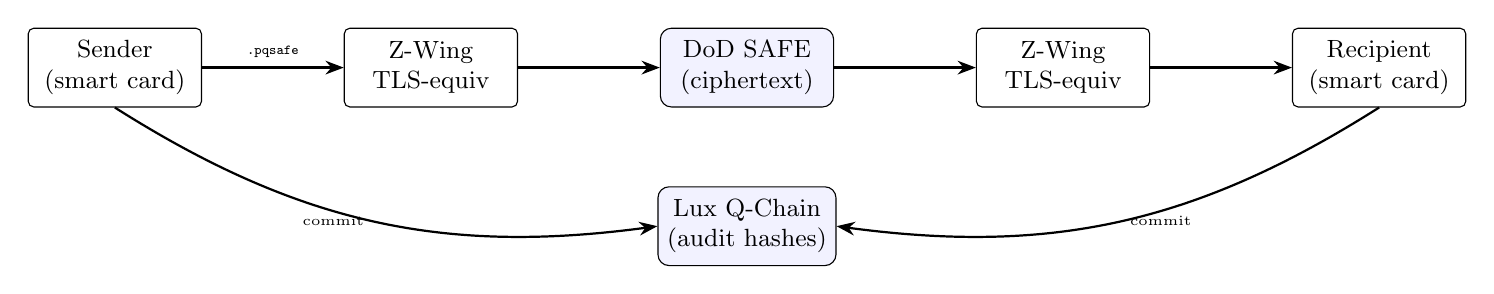
\begin{tikzpicture}[
  node distance=10mm and 18mm,
  every node/.style={font=\small},
  box/.style={draw, rounded corners=2pt, minimum height=10mm,
              minimum width=22mm, align=center},
  cloud/.style={draw, rounded corners=4pt, fill=blue!5,
                minimum height=10mm, minimum width=22mm, align=center},
  arrow/.style={-Stealth, thick}
]
\node[box] (sender) {Sender\\(smart card)};
\node[box, right=of sender] (zwing) {Z-Wing\\TLS-equiv};
\node[cloud, right=of zwing] (safe) {DoD SAFE\\(ciphertext)};
\node[box, right=of safe] (zwing2) {Z-Wing\\TLS-equiv};
\node[box, right=of zwing2] (recipient) {Recipient\\(smart card)};
\node[cloud, below=of safe] (qchain) {Lux Q-Chain\\(audit hashes)};

\draw[arrow] (sender)--(zwing) node[midway,above,font=\tiny]{\texttt{.pqsafe}};
\draw[arrow] (zwing)--(safe);
\draw[arrow] (safe)--(zwing2);
\draw[arrow] (zwing2)--(recipient);
\draw[arrow] (sender.south) to[bend right=20] node[midway,left,font=\tiny]{commit} (qchain.west);
\draw[arrow] (recipient.south) to[bend left=20] node[midway,right,font=\tiny]{commit} (qchain.east);
\end{tikzpicture}
\caption{Sender and recipient hold the only plaintext. Z-Wing protects
the channel; DoD SAFE / object storage / SharePoint / etc.\ holds
ciphertext; Q-Chain holds audit hashes only.}
\end{figure}

\subsection{Migration from DoD SAFE today}

DoD SAFE currently provides TLS-protected file drop-off with sender-set
expiry. The migration path:

\begin{enumerate}[leftmargin=*,itemsep=0pt]
\item \textbf{Phase 1 (PQSAFE alongside SAFE).} Users upload PQSAFE
  envelopes through SAFE unchanged. SAFE sees only ciphertext; the
  existing SAFE infrastructure is untouched.
\item \textbf{Phase 2 (PQSAFE-native ingest).} A \texttt{safe.apps.mil}
  endpoint accepts PQSAFE envelopes directly, fronted by Z-Wing for
  endpoint-to-endpoint PQ confidentiality and an HSM-backed
  certificate chain for ABAC enforcement.
\item \textbf{Phase 3 (legacy SAFE deprecation).} SAFE TLS-only mode is
  retired; \texttt{safe.apps.mil} requires either Z-Wing or
  PQSAFE-on-TLS-1.3-hybrid. Backward-compat preserved through the
  hybrid TLS cipher suite (X25519MLKEM768, IANA \texttt{0x11ec}).
\end{enumerate}

% ===========================================================================
\section{What we don't do}
\label{sec:nondoers}

\begin{itemize}[leftmargin=*,itemsep=0pt]
\item Don't say ``blockchain makes files secure.'' The chain is an
  audit anchor, nothing more.
\item Don't store plaintext, filenames, recipient identities, or
  passphrases on-chain.
\item Don't use PQ-only before the hybrid migration is policy-accepted.
\item Don't invent a new KEM, signature, or AEAD.
\item Don't treat DoD SAFE as PQ just because it uses TLS.
\item Don't treat Lux primitive claims as DoD-approved without
  FIPS~140-3 validation, code audit, SBOM, threat model, and ATO
  evidence.
\item Don't use Pulsar/Corona threshold consensus signatures as if
  they were file encryption.
\item Don't use smart contracts as a key manager for CUI/PII/PHI.
\end{itemize}

% ===========================================================================
\section{Conclusion}

PQSAFE-IL5-HYBRID-v1 is what DoD asks for when DoD says ``replace SAFE
with something post-quantum and crypto-agile.'' It is not a new
cryptosystem. It is a small layer of envelope discipline applied above
NIST-standardised primitives, with the Lux PQ stack supplying the
parts (Z-Wing for the channel, age + ML-KEM for at-rest, corona +
pulsar for threshold recovery, the Q-Chain for audit anchoring, KMS
for HSM-backed key custody). The win is not novelty -- it is that
\emph{every byte that leaves a DoD endpoint is encrypted with a hybrid
classical + post-quantum primitive that NIST has standardised, the
sender has signed, the manifest has bound, and the audit log has
witnessed, without trusting the storage system, the network, or the
auditor with anything beyond a hash}.

% ===========================================================================
\begin{thebibliography}{99}

\bibitem{fips203}
NIST. \emph{FIPS 203: Module-Lattice-Based Key-Encapsulation Mechanism
Standard.} August 2024.
\url{https://csrc.nist.gov/pubs/fips/203/final}

\bibitem{fips204}
NIST. \emph{FIPS 204: Module-Lattice-Based Digital Signature Standard.}
August 2024.
\url{https://csrc.nist.gov/pubs/fips/204/final}

\bibitem{fips205}
NIST. \emph{FIPS 205: Stateless Hash-Based Digital Signature Standard.}
August 2024.
\url{https://csrc.nist.gov/pubs/fips/205/final}

\bibitem{fips197}
NIST. \emph{FIPS 197: Advanced Encryption Standard (AES).} 2001 /
updated 2023.

\bibitem{sp800208}
NIST. \emph{Special Publication 800-208: Recommendation for Stateful
Hash-Based Signature Schemes.} October 2020.

\bibitem{cnsa2}
NSA. \emph{Commercial National Security Algorithm Suite 2.0
(CNSA 2.0).} September 2022.
\url{https://www.nsa.gov/Press-Room/Press-Releases-Statements/Press-Release-View/Article/3148990/}

\bibitem{xwing2024}
Manuel Barbosa, Deirdre Connolly, Jo\~ao Diogo Duarte, Aaron Kaiser,
Peter Schwabe, Karoline Varner, Bas Westerbaan.
\emph{X-Wing: The Hybrid KEM You've Been Looking For.}
IACR ePrint 2024/039 and
IETF \texttt{draft-connolly-cfrg-xwing-kem}.
\url{https://eprint.iacr.org/2024/039}

\bibitem{rfc8439}
Y. Nir, A. Langley. \emph{RFC 8439: ChaCha20 and Poly1305 for IETF
Protocols.} 2018.

\bibitem{rfc8949}
C. Bormann, P. Hoffman. \emph{RFC 8949: Concise Binary Object
Representation (CBOR).} 2020.

\bibitem{rfc8152}
J. Schaad. \emph{RFC 8152: CBOR Object Signing and Encryption (COSE).}
2017.

\bibitem{age}
Filippo Valsorda. \emph{age: A simple, modern and secure file
encryption tool, format, and Go library.}
\url{https://age-encryption.org/}

\bibitem{luxage}
Lux Industries Inc. \emph{luxfi/age: hybrid PQ recipient stanza for
age.}
\url{https://github.com/luxfi/age}

\bibitem{luxzwing}
Lux Industries Inc. \emph{luxfi/zwing: Z-Wing post-quantum secure
channel + canonical X-Wing / hybrid-identity primitives.}
\url{https://github.com/luxfi/zwing}

\bibitem{pqsafe}
Lux Industries Inc. \emph{luxfi/pqsafe: reference implementation of
PQSAFE-IL5-HYBRID-v1.}
\url{https://github.com/luxfi/pqsafe}

\bibitem{pqrns}
Lux Industries Inc. \emph{luxfi/pqrns: PQ-RNS hybrid post-quantum
profile for the Reticulum Network Stack.}
\url{https://github.com/luxfi/pqrns}

\bibitem{lp9701}
Lux. \emph{LP-9701: Reticulum Network Stack (RNS) — hybrid PQ profile.}
\url{https://github.com/luxfi/lps/blob/main/LPs/lp-9701-reticulum-network-stack.md}

\bibitem{lp019}
Lux. \emph{LP-019: Threshold MPC.}
\url{https://github.com/luxfi/lps/blob/main/LPs/lp-019-threshold-mpc.md}

\end{thebibliography}

\end{document}
